\documentclass[11pt]{article}
\usepackage{amsmath}
%\usepackage{extsizes}
\usepackage{amsmath,amssymb}
%\usepackage{omegavn,ocmrvn}
%\usepackage[utf8x]{inputenc}
\usepackage[utf8]{vietnam}

\usepackage{listings}
\lstset{language=Python}          % Set your language (you can change the language for each code-block optionally)


\usepackage{longtable}
\usepackage{answers}
\usepackage{graphicx}
\usepackage{array}
\usepackage{pifont}
\usepackage{picinpar}
\usepackage{enumerate}
\usepackage[top=3.0cm, bottom=3.5cm, left=3.5cm, right=2.5cm] {geometry}
\usepackage{hyperref}

\newtheorem{bt}{Câu}
\newcommand{\RR}{\mathbb R}
\Newassociation{sol}{Solution}{ans}
\newtheorem{ex}{Câu}
\renewcommand{\solutionstyle}[1]{\textbf{ #1}.}


\begin{document}
% \noindent

\begin{tabular*}
	{\linewidth}{c>{\centering\hspace{0pt}} p{.7\textwidth}}
	Trường ĐHKHTN, ĐHQGHN & {\bf Học Kỳ 2 (2021-2022)}
	\tabularnewline
	K64 TTƯD - Thầy Hà Phi & {\bf Bài Tập Giải Tích Số \\ \today}
	% Exercises on pages 239, 240 Cheney/Kincaid are really nice
	\tabularnewline
	\rule{1in}{1pt}  \small  & \rule{2in}{1pt} %(Due date:)
	\tabularnewline
	%  \tabularnewline
	%  &(Đề thi có 1 trang)
\end{tabular*}




\begin{center}
	{\bf Bài Tập Lý Thuyết Điều Khiển Hệ Thống - No. 1}
\end{center}

\begin{bt}
Bài toán 1 (con lắc ngược): Xét mô hình điều khiển của một con lắc ngược (sau khi được tuyến tính hóa) cho bởi một phương trình vi phân bậc hai
\begin{equation}\label{1}
\vphi"(t) - \vphi(t) = u(t).
\end{equation}
%
Ở đây, $\vphi(t) = \tet(t) - \pi$ là độ lệch góc của con lắc so với trạng thái cân bằng thẳng đứng tại thời điểm $t \geq 0$ và $u(t)$ là mômen lực tác dụng. \\ 
%
\begin{figure}[!h]
	\centering
	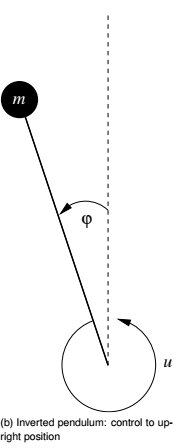
\includegraphics[scale = 0.7]{Figures/inverted_pendulum}
	\caption{Con lắc ngược - Điều khiển sao cho con lắc chuyển động hướng về trục thẳng đứng}
	\label{fig:invertedpendulum}
\end{figure}

\noindent  a) Chứng tỏ rằng đối với phản hồi tỷ lệ thuận (proportional state feedback) $u(t) = -\a \vphi(t)$ với $\a <1$, mệnh đề sau là đúng: 
Nếu các giá trị ban đầu thỏa mãn $\vphi'(0) = - {\vphi}(0)\sqrt{1-\a}$, thì $\underset{t\rar \infty}{\lim} \vphi(t) = 0$.
b) Cho $\a \in \R$ cố định. Xét hàm năng lượng $V(x,y):= cos x - 1 + \dfrac{1}{2} (\a x^2 +y^2)$. Chứng minh rằng $V(\vphi(t),\vphi'(t))$ là hằng số dọc theo các nghiệm của phương trình con lắc phi tuyến với phản hồi tỷ lệ thuận, được cho bởi
\begin{equation}\label{2}
	\vphi"(t) - \sin(\vphi(t)) + \a \vphi(t) = 0 \ .
\end{equation}
%
Từ đó kết luận rằng tồn tại các điều kiện ban đầu $\vphi(0)= \ep; \ \vphi'(0) = 0$ sao cho nghiệm của \eqref{2} với $\ep$ nhỏ tùy ý không thỏa mãn $\underset{t\rar \infty}{\lim} \vphi(t) = 0$, $\underset{t\rar \infty}{\lim} \vphi'(t) = 0$. \\
\end{bt}

\pagebreak

\begin{bt} \textbf{Bài tập về biến đổi Laplace để huẩn bị cho hàm truyền trong Bài Giảng 2.} \\
Biến đổi Laplace của 1 hàm số $x(t)$ được định nghĩa bởi
%
\[
X(s) := L[x(t)] = \int_0^{\infty} x(t) e^{-st} dt \ , 
\]
%
trong đó $s$ là 1 số phức với phần thực $\Re(s)<0$. Ta nói $X(s)$ là biến đổi Laplace của hàm $x(t)$. Biến đổi Laplace chuyển hàm từ miền thời gian $t$ (time domain) sang miền tần số $z$ (frequency domain). Chứng minh các tính chất sau của biến đổi Laplace. \\
a) Nếu $a$, $b$ là các hằng số thì $L[ax(t) + by(t)] = a X(s) + b Y(s)$. \\
b) $L[e^{-at}] = \dfrac{1}{s+a}$ \ . \\
c) $L[x'(t)] = s X(s) - x(0)$. \\
d) $L[x(t-\tau)] = e^{-s\tau} X(s)$. \\
e) $L[e^{-at} x(t)] = X(s+a)$. 
\end{bt}   

\begin{bt}
a) Hãy áp dụng biến đổi Laplace cho hệ LTI 
%
\begin{align}\label{3}
\dot{x}(t) &= A x(t) + B u(t), \notag \\
y(t) &= Cx(t) + Du(t),
\end{align}
%
để xây dựng công thức hàm truyền (transfer function) $G(s)$ sao cho $Y(s) = G(s) U(s)$.\\
b) Trong các mô hình điều khiển của 2 hệ thống điện được mắc nối tiếp và mắc song song hãy tìm mối liên hệ của hàm truyền hệ thống tổng với hàm truyền của 2 hệ thống con.

\begin{figure}[h!]
	\centering
	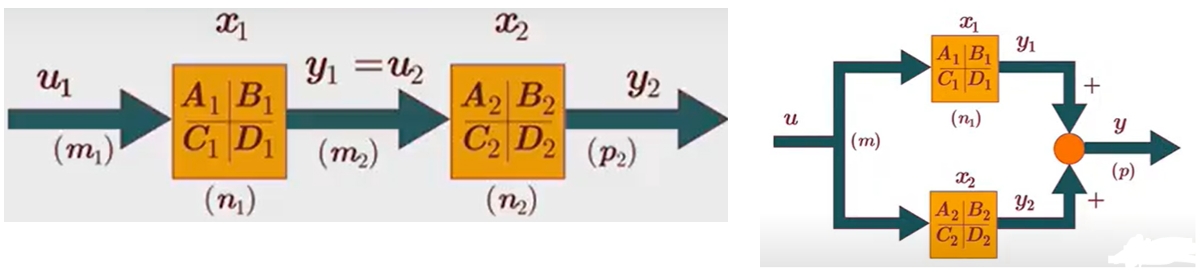
\includegraphics[scale = 0.6]{Figures/Electrical_connection}
	\caption{Mạch điện mắc nối tiếp (trái) và song song (phải).}
	\label{fig:fig1}
\end{figure}


\end{bt}

\begin{bt} 
a) Nhắc lại rằng hai phương trình $\dot{x}(t) = A(t) x(t)$	và $\dot{z}(t) = -A^T(t) z(t)$ là \emph{liên hợp}. Hãy tìm phương trình liên hợp của hệ LTV
%
\begin{equation}\label{3}
	\dot{x}(t) = A(t) x(t) + B(t) u(t).
\end{equation}
%
b) Cho họ tiến hóa của phương trình $\dot{x}(t) = A(t) x(t)$ là $\{\Phi(t,s)\}_{t\geq s}$. Hãy xác định họ tiến hóa của phương trình liên hợp $\dot{z}(t) = -A^T(t) z(t)$.
\end{bt}

\pagebreak

\begin{bt}
Cặp ma trận vuông $(E,A) \in (R^{n,n})^2$ được gọi là chính quy nếu $\det(sE-A) \not= 0$ với số $s\in C$ nào đó. Giả sử rằng cặp ma trận vuông $(E,A)$ là chính quy, hãy chứng minh các khẳng định sau. \\
a) Tồn tại 1 ma trận $K$ khả nghịch sao cho $KE$ và $KA$ là giao hoán. \\
b) Tồn tại 2 ma trận khả nghịch $W$, $T$ sao cho $WET = \m{I & 0 \\ 0 & N}$, $WAT = \m{J & 0\\ 0 & I}$ trong đó $J$ có dạng Jordan, $N$ là ma trận lũy linh. \\
c) Từ đó hãy tìm công thức nghiệm tường minh của phương trình 
%
\[
E \dot{x}(t) = A x(t) + f(t), 
\]
%
giả sử rằng hàm $f(t)$ là đủ trơn.
\end{bt}

\end{document}


\begin{bt} \textbf{(tính ổn định của hệ thống LTI):} Cho $A \in \R^{n,n}$. Chứng minh các khẳng định sau: \\
	a) PTVP $x'(t) = Ax(t)$ là ổn định tiệm cận khi và chỉ khi $\sigma(A) := \{ \lambda \in \C \ | \ \det(\lambda I-A) = 0\} \subset \C_{-}$ và $\sigma(A) \cap i\R = \emptyset$. \\
	b) PTVP $x'(t) = Ax(t)$ là ổn định khi và chỉ khi $\sigma(A) := \{ \lambda \in \C \ | \ \det(\lambda I-A) = 0\} \subset \C_{-}$ và các giá trị riêng thuần ảo là đơn (bội 1).
\end{bt}   

\begin{bt}
	a) Cho trước ma trận $A \in \R^{m,n}$. Chứng minh rằng $\|A\|_2 = \max\{\lambda \ | \ \det(\lambda I - A^TA) = 0 \}$. \\
	b) Cho ma trận $A \in \R^{n,n}$ khả nghịch, $B \in \R^{n,m}$, $C \in \R^{p,n}$, $D \in \R^{p,m}$. Chứng minh rằng $\m{A & B \\ C & D}$ khả nghịch khi và chỉ khi ma trận $M := D - CA^{-1}B$ là khả nghịch. \\
	c) Xét TH đặc biệt $p = m$ và $D \in \R^{m,m}$ là xác định âm. Chứng minh rằng ma trận $\m{A & B \\ B^T & D}$ là (nửa) xác định âm khi và chỉ khi $M$ là (nửa) xác định âm.
\end{bt}

\begin{bt} \textbf{Bài tập thực hành về tính ổn định - vẽ hình trong Matlab.}
Cho hệ \eqref{3} với các ma trận hệ số là 
%
\[
A = \m{1 & 1 \\ 4 & -2}, \ B = \m{1 & -1 \\ 1 & -1}, \ C = \m{1 & 0}, \ D = 0. 
\]
%
Hãy tìm hiểu các hàm \verb|eig| và \verb|ode45| trong MATLAB để xác định tính ổn định của hệ và vẽ hình 
đầu ra $y(t)$, trạng thái $x(t)$ với các dữ kiện sau:
%
\[
u(t) \mbox{ là hàm Heaviside (google nhé)}, \ x_0 = \m{1 \\ 1}, \ [t_0,t_f] = [0,10] \ .
\]
% 
\end{bt}
